\chapter{Matrix Element method} \label{ch::MW}

\section{MadWeight theory} \label{sec::MWTheory}

\section{Resolution functions} \label{sec::TF}

\paragraph{Update of Friday 16 October 2015 :} 
Important issue about the Transfer Functions discovered by looking at their distribution beyond the fitted range!
\\

The way the TF's were determined was by optimizing the fitted range and making sure that the fit corresponded well with the measured MC points. However this way there is no control about what happens beyond this range, and looking at the full fit function clearly indicated strange shapes and peaks in this area. This was also neatly visible in the comparison of the ``old'' and ``new'' TF's (b-jets mainly). 
\\
\textit{ \underline{Remark: } The strange behaviour of the ``old'' TF is not really understood. When looking at the individual fit distributions when creating these shapes the minimum was always positioned at the expected position.}
\begin{figure}[h!t]
 \centering
 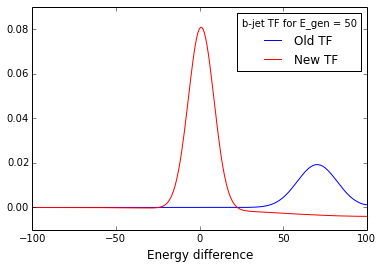
\includegraphics[width = 0.24 \textwidth]{Chapters/Chapter5_MadWeight/Figures/BJetTF_OldvsNew_Egen50.png}
 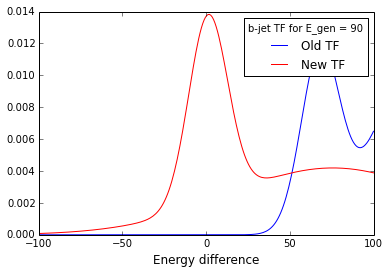
\includegraphics[width = 0.24 \textwidth]{Chapters/Chapter5_MadWeight/Figures/BJetTF_OldvsNew_Egen90.png}
 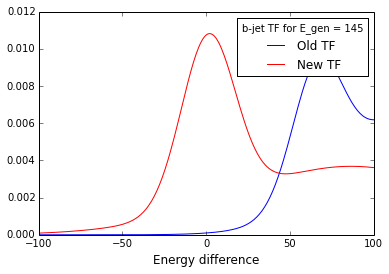
\includegraphics[width = 0.24 \textwidth]{Chapters/Chapter5_MadWeight/Figures/BJetTF_OldvsNew_Egen145.png}
 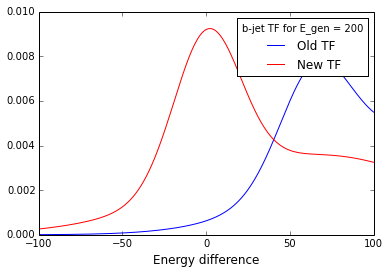
\includegraphics[width = 0.24 \textwidth]{Chapters/Chapter5_MadWeight/Figures/BJetTF_OldvsNew_Egen200.png}
 \caption{Comparison between the old (blue) and new (red) TF in order to understand why the former does give the correct minimum and the latter one not. From these plots a conclusion cannot really be made since it seems that none of them actually corresponds to the expected distribution. For the most recent one the additional peak at positive $\Delta E$ values should clearly dissapear.}
\end{figure}
\hfill \\
For this reason the method to determine the TF's has been adapted such that the full fit function is visible and not only the fit on the restricted range. In order to better visualize the tail and the double gaussian behaviour further from 0, the considered $\Delta E$ range has also been extended up to $-100$ and $100$. 
\\
This new approach indicates that the old method gave rise to completely wrong distributions and that the only way to capture the tail is by giving up the precise determination of the peak a little bit. For each of the $E_{gen}$ bins of the b-jet distribution the position of the main peak is slightly off, but in general the shape can be labelled acceptable (and results in decent parameter results).
\begin{figure}[h!t]
 \centering
 \includegraphics[width = 0.49 \textwidth]{Chapters/Chapter5_MadWeight/Figures/sliceYbin1And2_BJet_DiffEVsGenE.pdf}
 \includegraphics[width = 0.49 \textwidth]{Chapters/Chapter5_MadWeight/Figures/sliceYbin8_BJet_DiffEVsGenE.pdf}
 \includegraphics[width = 0.49 \textwidth]{Chapters/Chapter5_MadWeight/Figures/sliceYbin1And2_BJet_DiffEVsGenE_OLDRange.pdf}
 \includegraphics[width = 0.49 \textwidth]{Chapters/Chapter5_MadWeight/Figures/sliceYbin8_BJet_DiffEVsGenE_OLDRange.pdf}
 \caption{Upper plots are obtained with the new method (focus on shape outside fitted range) while lower ones are how the TF were created earlier (focus on good fit in range).}
\end{figure}
\hfill \\
When comparing these new TF's with the old ones, the strange shape on the positive side of $\Delta E$ completely dissapeared and now looks more like the expected distribution.
\begin{figure}[h!t]
 \centering
 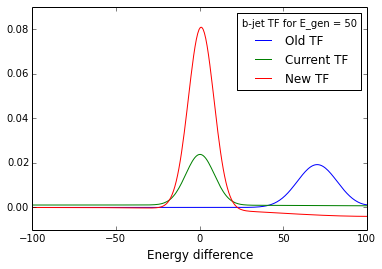
\includegraphics[width = 0.24 \textwidth]{Chapters/Chapter5_MadWeight/Figures/BJetTF_OldvsNewvsCurr_Egen50.png}
 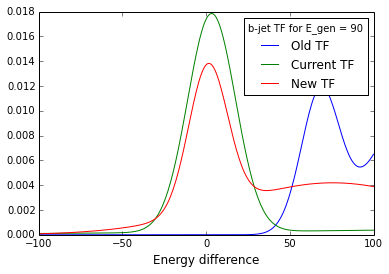
\includegraphics[width = 0.24 \textwidth]{Chapters/Chapter5_MadWeight/Figures/BJetTF_OldvsNewvsCurr_Egen90.png}
 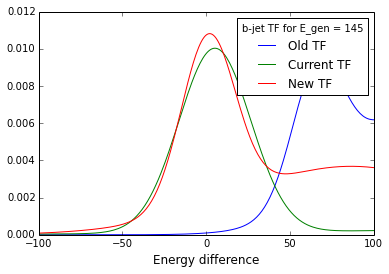
\includegraphics[width = 0.24 \textwidth]{Chapters/Chapter5_MadWeight/Figures/BJetTF_OldvsNewvsCurr_Egen145.png}
 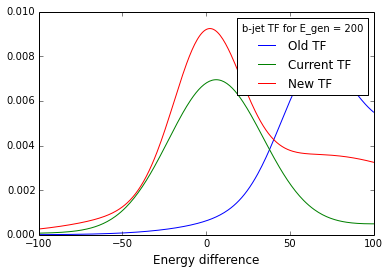
\includegraphics[width = 0.24 \textwidth]{Chapters/Chapter5_MadWeight/Figures/BJetTF_OldvsNewvsCurr_Egen200.png} 
 \caption{Overall distribution obtained for the new TF's for different $E_{gen}$ energies.}
\end{figure}
\hfill \\
To finalize the TF discussion for the b-jets, the obtained parameter distributions are given. These represent the obtained mean and width of the two gaussians and their relative weight in the fit formula. The results look rather stable, beside some fluctuations for the wide gaussian, which is also expected since this one can be determined not as precise as the narrow one. However the $E_{gen}$ bins where the wide gaussian is expected to be more important succeeded in measuring the required precise enough to do the fit. 
\\
The most thrustworthy result is obtained for the relative constant which clearly shows that the second gaussian only becomes significant for higher values of $E_{gen}$ since the $\Delta E$ distribution becomes significantly broader for these events. However it is also the region where the double gaussian shape matches best with the fitted MC points.
\begin{figure}[h!t]
 \centering
 \includegraphics[width = 0.32 \textwidth]{Chapters/Chapter5_MadWeight/Figures/BJet_DiffEVsGenE_a1_Fit.pdf}
 \includegraphics[width = 0.32 \textwidth]{Chapters/Chapter5_MadWeight/Figures/BJet_DiffEVsGenE_a2_Fit.pdf}
 \includegraphics[width = 0.32 \textwidth]{Chapters/Chapter5_MadWeight/Figures/BJet_DiffEVsGenE_a3_Fit.pdf}
 \includegraphics[width = 0.32 \textwidth]{Chapters/Chapter5_MadWeight/Figures/BJet_DiffEVsGenE_a4_Fit.pdf}
 \includegraphics[width = 0.32 \textwidth]{Chapters/Chapter5_MadWeight/Figures/BJet_DiffEVsGenE_a5_Fit.pdf}
\end{figure}

For some (currently unexplained) reason the result obtained for the light jets did not encounter the same issue and here the distributions for the ``old'' and ``new'' TF's were almost identically. Hence only effort has been awarded to the b-jet fixing in order to run a quick test whether this would already result in the expected outcome.
\begin{figure}[h!t]
 \centering
 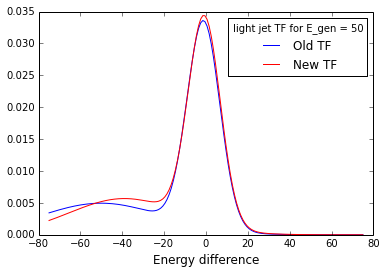
\includegraphics[width = 0.3 \textwidth]{Chapters/Chapter5_MadWeight/Figures/LightTF_OldvsNew_Egen50.png}
 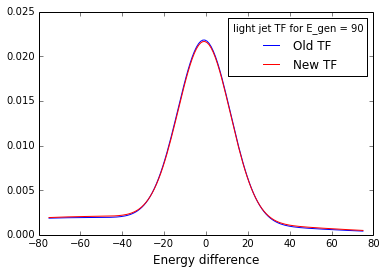
\includegraphics[width = 0.3 \textwidth]{Chapters/Chapter5_MadWeight/Figures/LightTF_OldvsNew_Egen90.png}
 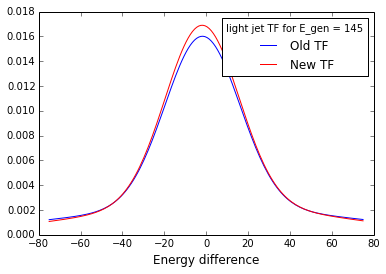
\includegraphics[width = 0.3 \textwidth]{Chapters/Chapter5_MadWeight/Figures/LightTF_OldvsNew_Egen145.png}
 \caption{Comparison of TF's for the light jets, which are clearly almost identical. Hence no update for these has been done for the moment.}
\end{figure}
\hfill \\
In order to be sure the light jets really behave properly, some examples of individual fit distributions have been added anyway. This indeed shows that the double Gaussian shape correctly takes both the peak and the tail. However some minor improvement can still be achieved in the negative side of the $\Delta E$ distribution for low values of $E_{gen}$. As a final cross-check the range of the muon distributions will also be extended up to $-75$ and $75$ in order to check whether some improvement can be reached, as was the case for the b-jet distributions.
\begin{figure}[h!t]
 \centering
 \includegraphics[width = 0.49 \textwidth]{Chapters/Chapter5_MadWeight/Figures/sliceYbin1And2_Light_DiffEVsGenE.pdf}
 \includegraphics[width = 0.49 \textwidth]{Chapters/Chapter5_MadWeight/Figures/sliceYbin8_Light_DiffEVsGenE.pdf}
 \caption{Fit distributions for light jets which again indicate that the original method works out-of-the-box for the light jets and do not experience the same strange behaviour as the b-jets.}
\end{figure}

For the moment, to quickly check the influence of these updated b-jet TF's, it has been decided to use delta-functions for the muons. However looking at the narrow $\Delta E$ distributions for the muon events, it is maybe sufficient to use delta-functions for the actual analysis.
%As a final remark, it has been decided to use delta-functions for the muons since this will be good enough. (Also paper of Kelly goes out with delta for muons and this will be made public...). 
In case electrons would be considered this however requires non-delta shaped TF's.\\
If really necessary the same procedure can be done in order to provide eta-binned TF's for both the b-jets and the light jets, but this will again require a lot of time ... And as long als the final TF's haven't been decided on, the full list of MC samples cannot be send through MadWeight!

\section{Generator-level results} \label{sec::GenResults}